% diagrams/english/biblioteca.tex -- el rincón inglés de la biblioteca,
% para "Where is it?": una estantería alta, la ventana con el sofá
% debajo, la mesita al lado del sofá, la alfombra y la balda baja del
% rincón en inglés.
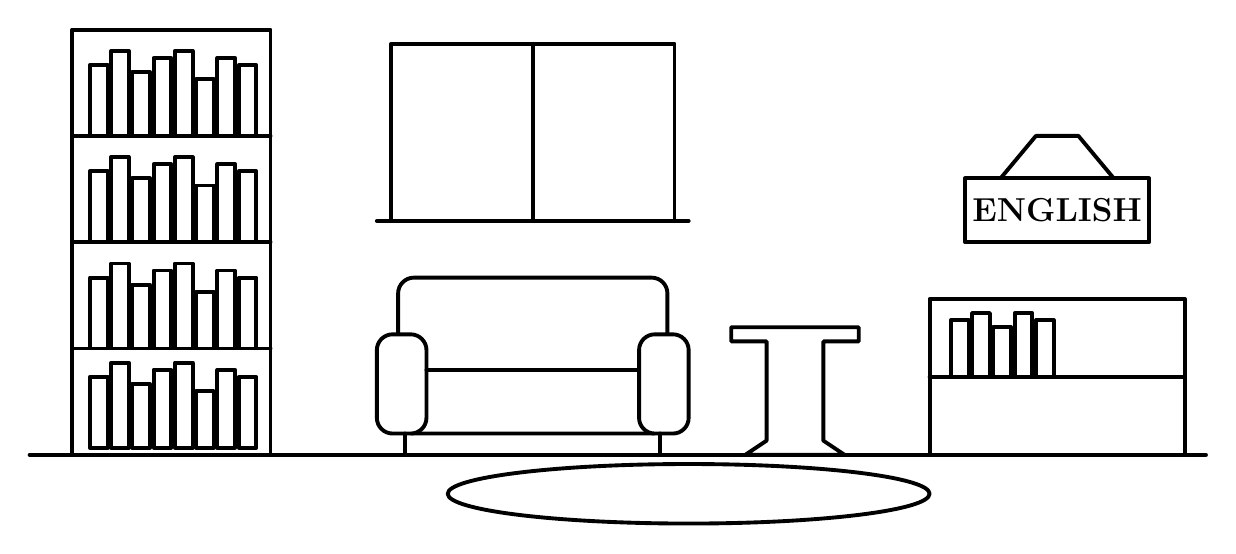
\begin{tikzpicture}[line width=1.4pt, line cap=round, line join=round, scale=0.9]
  \draw (-0.3,0) -- (16.3,0);
  % la estantería alta
  \filldraw[fill=white] (0.3,0) rectangle (3.1,6.0);
  \foreach \y in {1.5,3.0,4.5} { \draw (0.3,\y) -- (3.1,\y); }
  \foreach \b/\y in {0/1.5, 1/3.0, 2/4.5, 3/0.1} {
    \foreach \x/\h in {0.55/1.0,0.85/1.2,1.15/0.9,1.45/1.1,1.75/1.2,2.05/0.8,2.35/1.1,2.65/1.0} {
      \draw (\x,\y) rectangle ++(0.25,\h);
    }
  }
  % la ventana y el sofá verde, debajo
  \filldraw[fill=white] (4.8,3.3) rectangle (8.8,5.8);
  \draw (6.8,3.3) -- (6.8,5.8); \draw (4.6,3.3) -- (9.0,3.3);
  \filldraw[fill=white, rounded corners=2mm] (4.9,0.3) rectangle (8.7,2.5);
  \filldraw[fill=white, rounded corners=2mm] (4.6,0.3) rectangle (5.3,1.7);
  \filldraw[fill=white, rounded corners=2mm] (8.3,0.3) rectangle (9.0,1.7);
  \draw (5.3,1.2) -- (8.3,1.2);
  \draw (5.0,0.3) -- (5.0,0); \draw (8.6,0.3) -- (8.6,0);
  % la mesita, al lado del sofá
  \filldraw[fill=white] (9.8,0) -- (10.1,0.2) -- (10.1,1.6) -- (9.6,1.6) -- (9.6,1.8)
    -- (11.4,1.8) -- (11.4,1.6) -- (10.9,1.6) -- (10.9,0.2) -- (11.2,0) -- cycle;
  % la alfombra, en el suelo delante del sofá
  \filldraw[fill=white] (9.0,-0.55) ellipse (3.4 and 0.42);
  % la balda baja del rincón en inglés, con su cartel
  \filldraw[fill=white] (12.4,0) rectangle (16.0,2.2);
  \draw (12.4,1.1) -- (16.0,1.1);
  \foreach \x/\h in {12.7/0.8,13.0/0.9,13.3/0.7,13.6/0.9,13.9/0.8} { \draw (\x,1.1) rectangle ++(0.25,\h); }
  \filldraw[fill=white] (12.9,3.0) rectangle (15.5,3.9);
  \node[font=\bfseries\large] at (14.2,3.45) {ENGLISH};
  \draw (13.4,3.9) -- (13.9,4.5) -- (14.5,4.5) -- (15.0,3.9);
\end{tikzpicture}
